\documentclass{article}


\usepackage{arxiv}

\usepackage[utf8]{inputenc} % allow utf-8 input
\usepackage[T1]{fontenc}    % use 8-bit T1 fonts
\usepackage{hyperref}       % hyperlinks
\usepackage{url}            % simple URL typesetting
\usepackage{booktabs}       % professional-quality tables
\usepackage{amsfonts}       % blackboard math symbols
\usepackage{nicefrac}       % compact symbols for 1/2, etc.
\usepackage{microtype}      % microtypography
\usepackage{lipsum}
\usepackage{graphicx}
\usepackage{hyperref}
\usepackage{caption}

\title{Improving the state of retro console emulation}


\author{
  TheDot \\
  %Cody Morrison \\
  %Department of Computer Science\\
  %Personal Research\\
  %Calgary, AB \\
  %\texttt{codymorrison@thedanish.ca} \\
%  %% examples of more authors
%   \And
% Elias D.~Striatum \thanks{ASDFASDF}\\
%  Department of Electrical Engineering\\
%  Mount-Sheikh University\\
%  Santa Narimana, Levand \\
%  \texttt{stariate@ee.mount-sheikh.edu} \\
%  %% \AND
  %% Coauthor \\
  %% Affiliation \\
  %% Address \\
  %% \texttt{email} \\
  %% \And
  %% Coauthor \\
  %% Affiliation \\
  %% Address \\
  %% \texttt{email} \\
  %% \And
  %% Coauthor \\
  %% Affiliation \\
  %% Address \\
  %% \texttt{email} \\
}

\begin{document}
\maketitle

\begin{abstract}
\lipsum[1]
\end{abstract}


% keywords can be removed
\keywords{TAS \and Tool-Assisted Speedruns \and Emulation Accuracy \and Retro Gaming}


\section{Introduction}
Driven by a desire to improve the accuracy of emulation of  retro consoles, specifically the Nintendo Entertainment System (NES) and Super NES (SNES), we have implemented a system that allows the replay of Tool Assisted Speeduns (TAS’s) on real consoles.  TAS’s, if the reader is unfamiliar, are speedruns made on emulators making use of various tools available such as save states, viewing memory information to manipulate random number generation, enemy position, and various other things, as well as frame advance/slowdown to complete the game with the minimal amount of frames (and show off) while doing so.  Having been successful in the case of the NES, and partially successful in terms of the SNES, the author has been the first person to console verify a number of TAS’s, including but not limited to: NES Batman (http://youtu.be/AxkXrOu5IqQ) and NES Double Dragon 2(http://youtu.be/ieH539RaGKM).  


\section{Hardware}

Both replay devices are based on an Arduino uno, making use of 74h595c SIPO and 4021 PISO shift registers.  The 595 was selected due to being a well documented and commonly used shift register, and natively supported chaining which allowed for easy extension for multiple controllers on the NES as well as to the SNES replay device. Where as the 4021 was selected because it is the same shift register used in original NES and SNES controllers which allowed for easier integration

\subsection{NES}
The NES replay device was built using an Arduino uno, 1 74h595c SIPO shift register, and 1 4021 PISO shift register.   The 4021 was connected directly to the NES via 5 wires, $D0$. $V_{cc}$, $GND$, $LATCH$, $CLOCK$ in the same manner as a normal controller \ref{fig:NESReplay}, however as detailed later a 7 wire setup including D1 and D2 would be much more functional.  The 595 was connected so that the Most Significant Byte (MSB) was connected to the MSB of the 4021.  This was due to the way the data is stored for the NES, which is as a single byte per controller per frame in the order of ABSlStUDLR, where a zero represents the button being pushed and a 1 represents the button not being pushed on read. 

\begin{figure}
  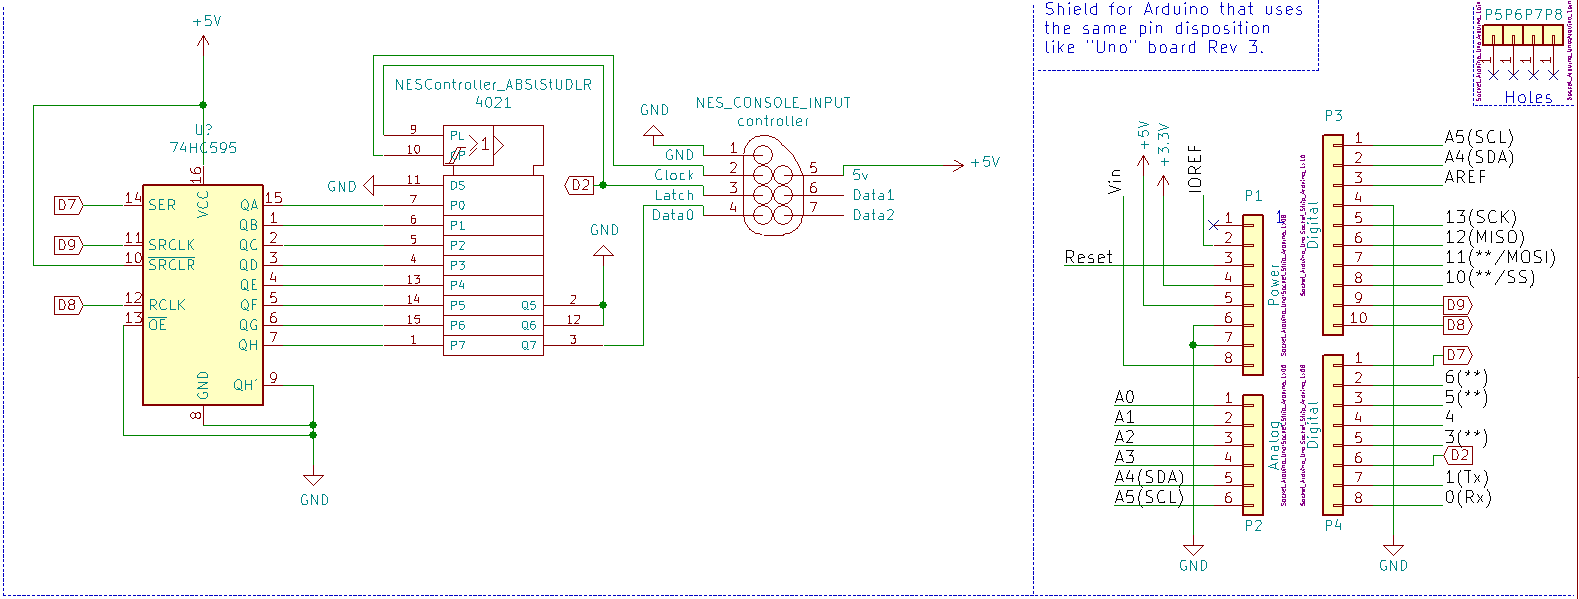
\includegraphics[width=\linewidth]{NESTASReplay.png}
  \caption{Electrical Diagram of NES Replay Device}
  \label{fig:NESReplay}
\end{figure}

\subsection{SNES}
The SNES replay device was built in a similar manner, using 2 74h595c registers, and 2 4021 registers.  They were daisy chained together, and the SNES has the same pins on the controller adaptor as the NES.  

\begin{figure}[h]
   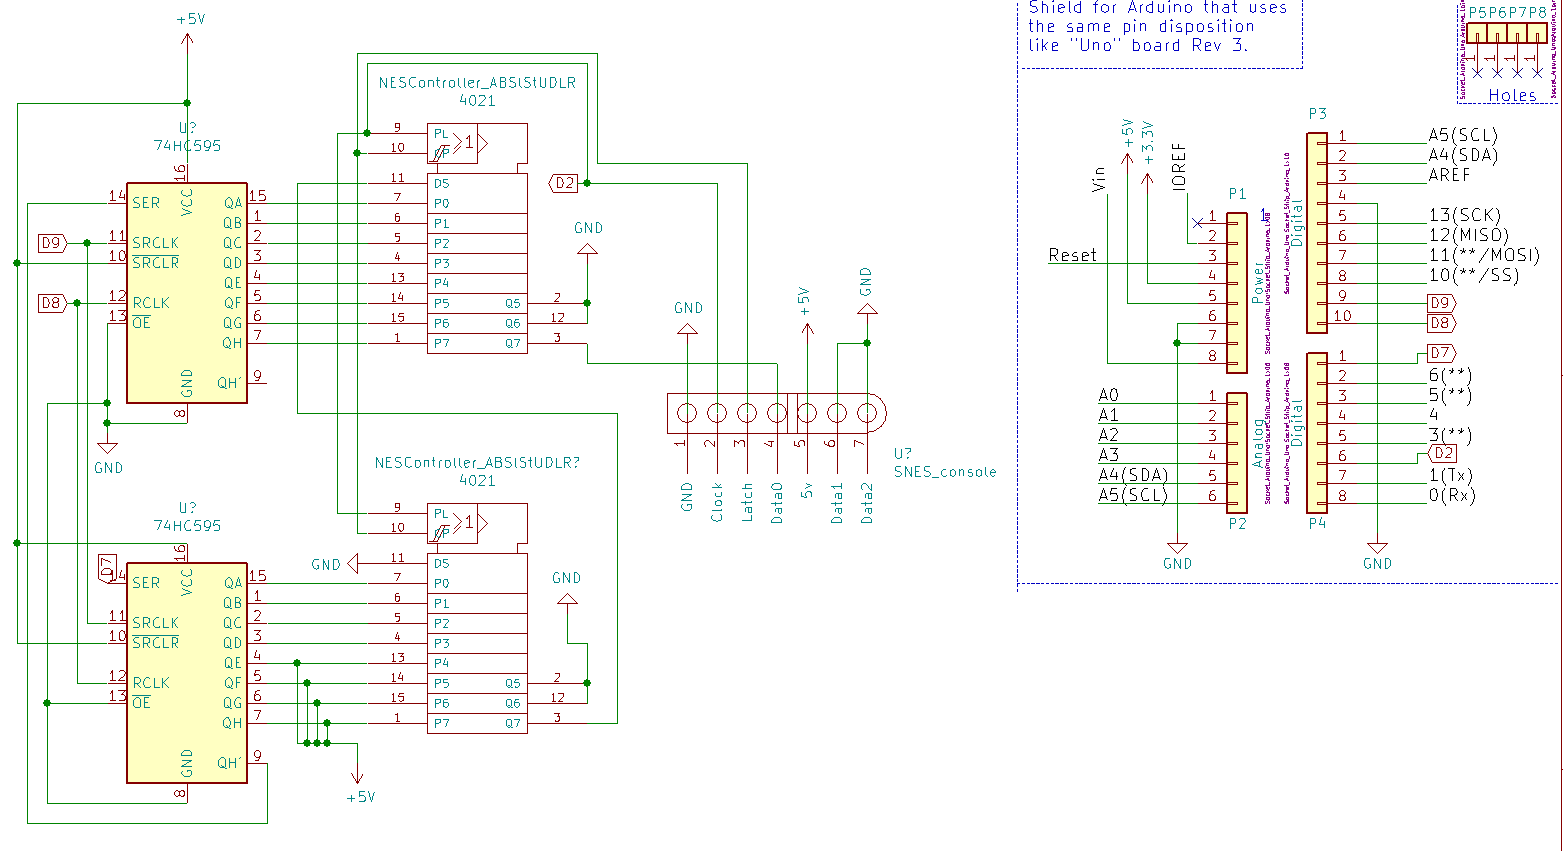
\includegraphics[width=\linewidth]{SNESTASReplay.png}
   \caption{Electrical Diagram of SNES Replay Device}
   \label{fig:SNESReplay}
\end{figure}

\section{Controller Protocol}
The arduino was programmed to accept information over a serial connection, and the controller latch wire was connected to an interupt to update the controller state.  A high level overview of the standard NES controller protocol and timing: Ideally once per frame the NES sends a 12$\mu$s long pulse on the latch line, then pulses the clock line 8 times and reads HIGH or LOW on the data line \ref{fig:NESControllerTiming}, and as shown in \ref{fig:SNESControllerTiming} the standard SNES controller is similar, with 16 clock pulses of which the last 4 are always high. The SNES controller layout is shown in \ref{fig:SNESController}, where the last four pulses on the DATA line are identification bits and always high for a standard controller, and the NES almost identical except it has only a single 4021 with A replacing B and B replacing Y.

\begin{figure}
    \includegraphics[width=\linewidth]{NESControllerProtocol.PNG}
    \caption{Timing diagram of NES Controller Protocol}
    \label{fig:NESControllerTiming}
\end{figure}

\begin{figure}
    \includegraphics[width=\linewidth]{SNESControllerProtocol.PNG}
    \caption{Timing diagram of SNES Controller Protocol}
    \label{fig:SNESControllerTiming}
\end{figure}


\begin{figure}[h]
   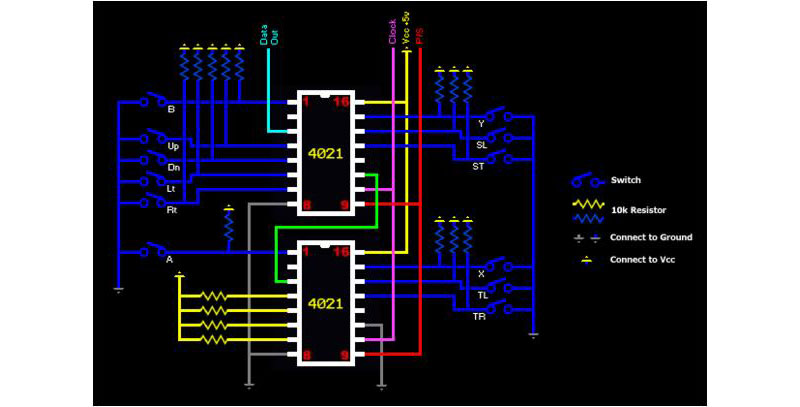
\includegraphics[width=\linewidth]{SNESController.jpg}
   \caption[]{ Electrical Diagram of SNES Controller\footnotemark}
   \label{fig:SNESController}
\end{figure}

\footnotetext{Benjamin Santiago: \href{https://www.digikey.com/en/maker/projects/diy-super-nintendo-breadboard-controller/788fd6f521824fb58715ca0b95b92840}{digikey}}

This is sufficient for a wide range of NES games including Super Mario Bros (SMB), Batman and sufficient for a small number of SNES games however there were several issues encountered during the build process, particularly surrounding audio on both the NES and SNES.    Some of these were surmountable, however the SNES has proven surprisingly troublesome to get working.  

\section{File format specification for r16m and r08}
The data that is sent to the arduino is first dumped from a tool assist movie file, generally using one of the dump scripts available \href{https://github.com/dwangoac/TASBot-Projects/tree/master/Dump_Scripts}{here}.  SNES movie files are saved in the r16m file format, whilst NES movie files are saved in the r08 file format.  These files are then parsed and sent via a serial connection to the arduino.  The file formats are detailed as follows, graciously provided by TheMas3212:
\begin{verbatim}
R08: 
2 Bytes per Frame 
Byte 1: Player1
Byte 2: Player2 

Bits        Hex     Buttons Pressed
00000000    00      no buttons pressed
11111111    ff      all buttons pressed

10000000    80   A Button
01000000    40   B Button
00100000    20   Select
00010000    10   Start
00001000    08   Dpad Up
00000100    04   Dpad Down
00000010    02   Dpad Left
00000001    01   Dpad Right

==================================================================

R16M
16 Bytes per Frame
Byte 1,2: Player1-1
Byte 3,4: Player1-2
Byte 5,6: Player1-3
Byte 7,8: Player1-4
Byte 9,10: Player2-1
Byte 11,12: Player2-2
Byte 13,14: Player2-3
Byte 15,16: Player2-4

Bits                Hex    Buttons Pressed
00000000 00000000   0000   no buttons pressed
11111111 11111111   ffff   all buttons pressed
11111111 11110000   fff0   all normal buttons pressed

10000000 00000000   8000   B Button
01000000 00000000   4000   Y Button
00100000 00000000   2000   Select Button
00010000 00000000   1000   Start Button
00001000 00000000   0800   Dpad Up
00000100 00000000   0400   Dpad Down
00000010 00000000   0200   Dpad Left
00000001 00000000   0100   Dpad Right

00000000 10000000   0080   A Button
00000000 01000000   0040   X Button
00000000 00100000   0020   L Button
00000000 00010000   0010   R Button
00000000 00001000   0008   1 Button
00000000 00000100   0004   2 Button
00000000 00000010   0002   3 Button
00000000 00000001   0001   4 Button

\end{verbatim}


\section{Issues}

\subsection{NES}

The NES makes use of DMC (delta modulation channel) to play back audio samples from memory, however due to a hardware issues in the 2A03 (the NTSC NES PPU) when using Direct Memory Access (DMA) it can corrupt the controller polling.  Exactly how this occurs in unclear, but the proposed reasoning is that the PPU pulls /RDY low on the CPU, but the clock signal keeps triggering causing the controller to shift out data that isn’t read, causing invalid data to be read from the controller.   This issue was supposedly fixed in the 2A07 which was used in the PAL release of the NES.  

There were several techniques implemented to deal with this issue; Super Mario Bros. 3 (SMB3) for example reads the controller twice and if the input matches then it passes control back to the main game cycle, otherwise it reads another pair of inputs.  Due to this, as well as the fixed sized buffer they use to store the controller reads, it is possible to overflow the buffer and achieve arbitrary code execution (ACE) on the NES however this requires a 7 wire cable due to the use of D1 and D2 for enhanced transfer speed.  For the unfamiliar, an ACE is when arbitrary data can be input by the user which is then executed by the device as valid code, instead of being treated as data, allowing the user to execute any code they like.
	
The solution for this was determined to be (thanks to the TASBot discord\footnote{\href{http://discord.tasbot.net/}{http://discord.tasbot.net/}}) to implement a window mode for controller reads.  Specifically for trouble titles using DMC audio you have arduino wait for at least X milliseconds to occur between latches, where X is dependent on the game.  SMB3 required an approximately 9 ms window, whilst Rescue Rangers required a 4 ms window.  No better way than simple brute force has been found to help narrow down the window as of yet. After implementation of the window mode several SMB3 runs were tested, including an ACE,\href{tasvideos.org/2588M.html}{2588M}, that required only D0 and was successful in testing, as well as any\% warps \href{tasvideos.org/3812M.html}{3812M}.  Complete syncing of any\% no-warp and 100\% are currently on going tasks, both have issues approximately 30 minutes into the run which may be an issue with the serial communication window and limited resources of an Arduino Uno, however PSoC5 based TAS replay devices have proven capable of syncing these runs as shown on the tasvideos website.  Non-DMC games appear to have no issues syncing regardless of length.  

\subsection{SNES}
The SNES has been particularly interesting and challenging to work on.  A limited number of games including Super Mario World are known to be relatively easy to sync; however due to the use of a ceramic oscillator for the APU, a quartz oscillator for the CPU and the fact that some SNES games wait for certain audio signals to finish before the CPU advances have resulted in difficulty getting many games to sync beyond a few seconds.  Several options have been attempted to increase the chances of syncing, including replacing the ceramic oscillator with a high quality quartz oscillator, however none of have been succesful.  Future endeavours will most likely include replacing both oscillators with a high quality clock signal generator and using a clock divider to control the speeds of the APU and CPU, and then adjusting the most accurate SNES emulator, \href{https://byuu.org/emulation/bsnes/}{bsnes}, to have clock speeds that match followed by resyncing the various TAS's in the emulator.


\bibliographystyle{unsrt}  
%\bibliography{references}  %%% Remove comment to use the external .bib file (using bibtex).
%%% and comment out the ``thebibliography'' section.


%%% Comment out this section when you \bibliography{references} is enabled.
\begin{thebibliography}{1}

\bibitem{TASBotDiscord}
\newblock The TASBot discord channel \#tasbot-dev was exceptionally helpful in researching and prototyping of the arduino solution

\bibitem{NESDevWiki}
\newblock The NESDev wiki, \href{http://wiki.nesdev.com/w/index.php/Nesdev_Wiki}{here}

\bibitem{SFCDevWiki}
\newblock The SFC Dev Wiki, \href{https://wiki.superfamicom.org/}{here}

\bibitem{Higan/BSNES}
\newblock Higan/BSNES source code for investigating desync issues on SNES, available \href{https://byuu.org/}{here}

\bibitem{dwangogit}
\newblock dwangoAC's github repository for TASBOT-Projects, available \href{https://github.com/dwangoac/TASBot-Projects}{here}

\bibitem{theDotGithub}
\newblock My arduino code and serial transfer code will be available on my github page shortly. 

\bibitem{This section will be filled out as I figure out everything I referenced}
\newblock Most of what I learned was from careful observation of a logic analyzer and oscilloscope, as well as advice of various people on the TASBot discord.  

%\bibitem{kour2014real}
%George Kour and Raid Saabne.
%\newblock Real-time segmentation of on-line handwritten arabic script.
%\newblock In {\em Frontiers in Handwriting Recognition (ICFHR), 2014 14th
%  International Conference on}, pages 417--422. IEEE, 2014.
%
%\bibitem{kour2014fast}
%George Kour and Raid Saabne.
%\newblock Fast classification of handwritten on-line arabic characters.
%\newblock In {\em Soft Computing and Pattern Recognition (SoCPaR), 2014 6th
%  International Conference of}, pages 312--318. IEEE, 2014.
%
%\bibitem{hadash2018estimate}
%Guy Hadash, Einat Kermany, Boaz Carmeli, Ofer Lavi, George Kour, and Alon
%  Jacovi.
%\newblock Estimate and replace: A novel approach to integrating deep neural
%  networks with existing applications.
%\newblock {\em arXiv preprint arXiv:1804.09028}, 2018.

\end{thebibliography}


\end{document}